\documentclass[11pt, titlepage, a4paper]{article}


\usepackage[hidelinks]{hyperref} % For clickable links
\usepackage{graphicx} % For images
\graphicspath{ {./graphics/} }
\usepackage[acronym]{glossaries}
\usepackage[automake]{glossaries-extra}
\usepackage[utf8]{inputenc} % For special characters
\usepackage[english]{babel} % For language-specific hyphenation patterns

\usepackage{enumitem}
\usepackage[]{datetime2}
\usepackage[a4paper, total={16.0cm, 25cm}]{geometry}
\usepackage[backend=biber, style=ieee, sorting=none]{biblatex}
\addbibresource{Internship.bib} % Imports bibliography file+
\def\labelitemi{--}
\usepackage[T1]{fontenc}
\usepackage{inconsolata}
\usepackage{float}
\usepackage[toc,page]{appendix}

\usepackage{color}
\usepackage{caption}
\newcommand{\source}[1]{\caption*{Source: {#1}} }

\definecolor{pblue}{rgb}{0.13,0.13,1}
\definecolor{pgreen}{rgb}{0,0.5,0}
\definecolor{pred}{rgb}{0.9,0,0}
\definecolor{pgrey}{rgb}{0.46,0.45,0.48}

\usepackage{listings}
\lstset{language=Java,
  showspaces=false,
  showtabs=false,
  breaklines=true,
  showstringspaces=false,
  breakatwhitespace=true,
  commentstyle=\color{pgreen},
  keywordstyle=\color{pblue},
  stringstyle=\color{pred},
  basicstyle=\ttfamily,
  moredelim=[il][\textcolor{pgrey}]{},
  moredelim=[is][\textcolor{pgrey}]{\%\%}{\%\%}
}

\setabbreviationstyle[acronym]{long-short}


\title{Internship Report}
\author{Emily Sterthaus \\ Matriculation Number: 451 342 \\ \href{mailto:m_ster15@uni-muenster.de}{m\_ster15@uni-muenster.de}\\ \\
\small Ifgi Supervisor: \href{mailto:christian.knoth@uni-muenster.de}{Christian Knoth}\\ \small con terra Supervisor: \href{mailto:t.fechner@conterra.de}{Thore Fechner}
}
\date{\today}
\newcommand{\myparagraph}[1]{\paragraph{#1}\mbox{}\\}
\setcounter{secnumdepth}{5}
\setcounter{tocdepth}{5}
\makeglossaries
\newacronym{gd}{GD}{Geologischer Dienst}
\newacronym{exif}{EXIF}{Exchangeable Image File Format}
\newacronym{iptc}{IPTC IIM}{International Press Telecommunications Council Information Interchange Model}
\newacronym{csw}{CSW}{Catalogue Service for the Web}
\newacronym{dz}{DZ-Gefahr}{Digitaler Zwilling - Gefahr}
\newacronym{fme}{FME}{Feature Manipulation Engine}
\newacronym{thw}{THW}{Technisches Hilfwerk}
\newacronym{bhkg}{BHKG}{Gesetz über den Brandschutz, die Hilfeleistung und den Katastrophenschutz}
\newacronym{kritis}{KRITIS}{Kritische Infrastrukturen}
\newacronym{crud}{CRUD}{CREATE, READ, UPDATE, DELETE}
\newacronym{rcp}{RCP}{Representative Concentration Pathways}
\newacronym{nrw}{NRW}{North Rhine-Westphalia}
\newacronym{dam}{DAM}{Data Asset Managment}
\newacronym{pdf}{PDF}{Portable Document Format}
\newacronym{tiff}{TIFF}{Tagged Image File Format}
\newacronym{gdinw}{GDI-NW}{Geodateninfrastruktur Nordrhein-Westfalen}
\newacronym{lvn}{LVN}{IT-Infrastruktur und Landesverwaltungsnetz}
\newacronym{bkg}{BKG}{Bundesamt für Kartographie und Geodäsie}
\newacronym{etrs89}{ETRS89}{European Terrestrial Reference System 1989}
\newacronym{pei}{PEI}{Peripheral Equipment Interface}
\newacronym{pdu}{PDU}{Protocol Data Unit}
\newacronym{css}{CSS}{Cascading Style Sheets}
\newacronym{zamg}{ZAMG}{Zentralanstalt für Meteorologie und Geodynamik}
\newacronym{gba}{GBA}{Geologische Bundesanstalt}
\newacronym{netcdf}{NetCDF}{Network Common Data Format}
\newacronym{gui}{GUI}{Graphical User Interface}
\newacronym{iso}{ISO}{International Organization for Standardization}
\newacronym{tls}{TLS}{Transport Layer Security}
\newacronym{ogc}{OGC}{Open Geospatial Consortium}
\newacronym{s3}{S3}{Simple Storage Service}
\newacronym{ipcc}{IPCC}{Intergovernmental Panel on Climate Change}
\newacronym{gdide}{GDI-DE}{Geodateninfrastuktur Deutschland}
\newacronym{inspire}{INSPIRE}{Infrastructure for Spatial Information in the European Community}

\newglossaryentry{fastapi}
{
        name=FastAPI,
        description={FastAPI is a modern, fast  web framework for building APIs with Python, leveraging type hints and asynchronous programming for efficient development.}
}

\newglossaryentry{postgres}
{
        name=PostgreSQL,
        description={PostgreSQL is an open-source relational database management system known for its reliability, robust feature set, and extensibility, widely used for handling structured data in various applications.}
}
\newglossaryentry{vue}
{
        name=Vue,
        description={Vue is an open-source progressive JavaScript framework for building websites and applications.}
}
\newglossaryentry{vuetify}
{
        name=Vuetify,
        description={Vuetify is a component framework for Vue that follows Material Design principles. Its aim is to provide all the necessary tools to create visually appealing and content-rich applications.}
}
\newglossaryentry{vite}
{
        name=Vite,
        description={Vite is a build tool that offers a faster and leaner development experience for modern web projects. It provides features such as extremely fast Hot Module Replacement and enhancements over native ECMAScript modules.}
}
\newglossaryentry{springboot}
{
        name=Spring Boot,
        description={Spring Boot simplifies the creation of stand-alone Spring-based applications that can be run with minimal Spring configuration, starter dependencies, and production-ready features, without the need for code generation or XML configuration.}
}
\newglossaryentry{azure}
{
        name=Microsoft Azure,
        description={Microsoft Azure is a cloud computing platform operated by Microsoft. It provides access to application and service management and development.}
}
\newglossaryentry{maven}
{
        name=Apache Maven,
        description={Maven is an open-source build tool written in Java that simplifies the management of multiple projects by handling build, reporting, and documentation from a central project object model.}
}
\newglossaryentry{redis}
{
        name=Redis,
        description={Redis is an open source, in-memory data structure store used as a database, cache, message broker, and streaming engine.}
}
\newglossaryentry{nginx}
{
        name=Nginx,
        description={Nginx is an open-source web server used for serving static or dynamic websites, reverse proxy, load balancing, and other HTTP and proxy server capabilities.}
}
\newglossaryentry{solr}
{
        name=Apache Solr,
        description={Apache Solr is an open-source enterprise search platform built on the Java library called Lucene. It provides full-text search, hit highlighting, faceted search, real-time indexing, dynamic clustering, database integration, and rich document handling.}
}
\begin{document}



\maketitle
\newpage
\tableofcontents
\newpage

\section{Introduction}

\subsection{Company Profile}
% con terra is a geo-IT company based in Münster, Germany. The company primarily develops customer-specific GeoIT solutions based on the \gls{fme} and various Esri technologies, such as ArcGIS. For this reason, con terra is an Esri Platinum Partner and the main distribution partner of Safe Software for \gls{fme}.

con terra is a German company specializing in Geo-IT solutions. Founded in 1993, it is headquartered in Münster, Germany. The company's primary focus is on integrating intelligent Geo-IT solutions into the IT infrastructures of various customers, both in the private sector and in public administration agencies. This integration enables efficient, cost-effective, and transparent utilization of geoinformation, thereby enhancing the efficiency of company processes.

A key aspect of con terra's operations is its partnership with Esri Inc., through which it backs the ArcGIS technology. The company enhances this technology with additional products and technologies, such as \gls{fme}, and the ERP platform SAP HANA, to meet specific needs. Their cooperation with universities and participation in research and development projects, standardization procedures, and committees of organizations like \gls{iso}, \gls{gdide}, \gls{ogc}, and \gls{inspire}, positions them to both influence and quickly adapt to market trends.

con terra's own products are primarily map.apps and smart.finder. Each with several add-ons and configurations, for example smart.finder - SDI or map.apps ETL. As an alternative, they are also working on an open source framework called Open Pioneer.

con terra has expertise in multiple sectors, including insurance, natural and environmental resources, telecommunications, trade, SDI and e-government, and real estate. Customer are for example TenneT TSO,  \gls {gd} \gls{nrw}, IT.NRW or the Bundesanstalt für Geowissenschaften und Rohstoffe  (BGR).

The company has a team of over 220 professionals from diverse fields, including computer science, geoscience, mathematics, physics, engineering, and ecology. %con terra prioritises a corporate culture based on values such as responsibility, humanity, individuality, and professionalism, which are integral to its business operations and customer relationships.

%The con terra also has a lot of benefits for its Employees, such as modern offices, a focus on Work-Life Balance with Flexible working hours, providing a company car or a jobbike. They also have huge focus on social events for example: Teamevents, con terra afternoons, Summer festival/Christmas party and a boathouse on the werse which can be rented


%The company employs over 220 professionals from diverse fields, including computer science, geoscience, mathematics, physics, engineering, and ecology. con trra prioritises a corporate culture based on values such as responsibility, humanity, individuality, and professionalism, which are integral to its business operations and customer relationships.

The con terra offers several benefits to its employees, including modern offices, a focus on work-life balance with flexible working hours, and the provision of a company car or job bike. The company also places a significant emphasis on social events, such as team events, con terra afternoons, summer festivals, Christmas parties, and a boathouse on the Werse that can be rented \cite{conterraUnternehmensubersicht2024}.





\subsection{Motivation}
As a Master's student in Geoinformatics and Spatial Data Science, my internship at con terra is a strategic step in my professional development. I have previous work experience with the company and am familiar with its standing as a leading geospatial software provider in Münster. This familiarity enables me to integrate seamlessly into the team and contribute effectively from the onset. The internship's focus on software development aligns perfectly with my academic training, offering a chance to apply theoretical knowledge in a practical setting. My objective for this internship is to improve my software development skills further. I plan to leverage the opportunities at con terra to enhance my technical expertise in geospatial IT.

\subsection{Internship Meta Information}

My internship at con terra was in Münster. It started on 01.09.2023 and ended on 31.03.2024. I was part of the Open Data and Copernicus team and the SDI \& E-Government department. I worked an average of 32 hours per week, partly in the office and partly remotely.

\section{Internship Content}
The projects i worked on in my internship differ from the ones specified in the Learning Agreement. The only project from the learning agreement that i actually participated in were the \gls{gd} \gls{nrw} Meta-\gls{dam} Portal Project. My participation in the Open Pioneer \cite{conterraOpenPioneerTrails2024} project was shifted to the \gls{dz} project as the Open Pioneer Project was not able to provide the necessary technological capabilities (3D visualization with proper administrative CRS support). As an alternative (in order to reach the learning agreement goals) the focus was shifted to the \gls{dz} project.
%were deemed infeasible. Therefore, I participated in the \gls {dz} project and in the Geosphere project.
%My internship was clearly structured. This took the form three different Projects, each in their own timeframe and with their own requirements.

\subsection{\glsxtrfull{gd} \gls{nrw} -  Meta-\glsxtrfull{dam} Portal }
\subsubsection{Introduction}
The  \gls {gd} \gls {nrw}  is the central geoscientific institution of \gls {nrw}. Their  core tasks are geoscientific mapping and the provision of geodata for administration, business and science \cite{GeoDatenFurNordrheinWestfalen2024}.
They have a wide range of assets, which are currently managed by a software called cumulus. As the used software is outdated, it does not meet the current requirements.

Primarily they  are required to make all data, where it is legally possible, open data \cite{GesetzZurForderung2017}.
Additionally, the GeolDG also requires the \gls{gd} to make their accessible by the public \cite{GesetzZurStaatlichen2020}.

Therefore, the main goal of this project was to conceptualize a new system and to implement a prototype of it.
\subsubsection{As-is Status}
The \gls{gd} digital archive contains over 450,000 assets. Assets in this context are for example images, \gls{pdf}, \gls{tiff} or videos. However, any digital file can be an asset. The total data volume is over 2 terabytes.
These assets are currently located on a shared drive and can be managed via the file system. The Cumulus software primarily manages the metadata associated with the assets. Currently, the \gls{gd} does not use any known metadata schema, but instead uses a list of custom attributes, such as Rating, Special Instructions and Label.
They also use \gls{exif} and \gls{iptc} metadata information for images, which is not managed by Cumulus. Instead, this is done with an additional software component. %Likely Irfanview 
The main issue with the Cumulus software is that the current local installation is no longer supported. The modern version of Cumulus is a cloud-based solution that cannot be used by the \gls{gd} due to legal restrictions.

% \subsubsection{The new system}
% The new system exists maninly as a concept. But a few features were already implemented as a prototype for the \gls{gd} to test them.
\subsubsection{Requirements}
The new system should eliminate the inadequacies of the old system. Therefore, a list of Requirements were collected. In the following there is a subset example of the main functional requirements:
\begin{itemize}
    \item Keeping the Internal metadata attributes (and adding new ones)
    \item Connection to the GEOportal.NRW
    \item \gls{crud} Operations for Datasets and associated metadata
    \item  Integrated Permission System
    \item (Multi-)Edit User-Interface for Metadata
    \item Sharing data
    \item Update \gls{exif} and \gls{iptc} Metadata when an update occurs
    \item Syncing/Translating Internal Metadata to \gls{iso} 19115 \cite{isoISO1911512014}/\gls{iso} 19119 \cite{isoISO191192016}
    \item Different Search Operations
\end{itemize}



In addition, there are quality requirements that focus on data integrity and the tech stack used. The software should be able to run on the cloud or a dedicated machine, and the data should be stored on a \gls{s3} or the file system. The system should also support an exit strategy.

A final requirement is that the system needs to be split. It should mainly run on the servers of  \gls{gd} \gls {nrw}. But  non-sensitive data should be hosted also publicly by IT.NRW.

\subsubsection{Technical Aspects}
To meet these requirements the smart.finder SDI was chosen as base software. As it can not meet all requirements standalone (for example it can only work with \gls{iso} 19115/\gls{iso} 19119, INPSIRE \cite{temporarymiwp2021-2024sub-group2.3.1TechnicalGuidanceImplementation} or \gls{gdide} Metadata \cite{gdi-dearbeitskreismetadatenArchitekturGeodateninfrastrukturDeutschlandKonventionen}) new software components were conceptualized and implemented to meet the designated requirements \cite{conterraSmartFinderSDI}.



As seen in \ref{fig:components} and \ref{fig:deployment} the new Software consists of a gd-nrw-api, gd-nrw-dam-smartfinder-sdi, gd-nrw-dam and gd-nrw-datastore.
In the following each software component will be shortly described:

The main part of the System is the smart.finder SDI, which is called gd-nrw-dam-smartfinder-sdi. It consists of several components which are listed below:
\begin{description}
    \item[smartfinder-search]: This component is responsible for managing data. It operates on an integrated Apache \Gls{solr} instance to enable the search and filter capabilities of the smartfinder. It also enables features such as full-text search, geo-searches, and filtering for specific attribute values.
    \item[smartfinder-editor]: This component represents the smart.editor, which enables the editing of Metadata in compliance with \gls{iso} 19115/\gls{iso} 19119, \gls{inspire}, or \gls{gdide}.
    \item[smartfinder-csw]: This component serves as the \gls{csw} interface, enabling the dissemination of data to other portals, including the GEOportal.NRW.
    \item[smartfinder-sdi]: This component constitutes the user interface for searching and accessing datasets.
          %\item[gd-nrw-dam-portal]: This component is an adapted version of the smartfinder-sdi component.

\end{description}
%Additional there are completely new Software Components that needs to be solely for the \gls{gd} developed. These software components are listed below: 
The final system then consists of the following components:
\begin{description}
    \item[gd-nrw-dam-portal]: This component is the altered version of the smartfinder-sdi for \gls{gd} interns.
    \item[gd-nrw-datastore]: This component is responsible for the raw data access. It has the ability to function with both the raw file system and \gls{s3}. It offers fundamental \gls{crud} capabilities for the data.
    \item[gd-nrw-dam]:  This component offers \gls{crud} functionality for metadata, including a frontend for Multi-Edit Metadata and Editing Single Metadata. %This component stores the metadata and manages the communication between the newly developed software components and the smartfinder-sdi. 
    \item[nrw-dam-portal]: This component is the public portal hosted by IT.NRW.

\end{description}



%The general workflow for documents is that all editing is done by \gls{gd} Staff, therefore their component handle all editing.

As the \gls{gd}  wanted to keept its own Attributes, an additional database was required to save these Attributes. The main database is called gd-nrw-datastore. As the data should also be partial public there is an additional databse at IT.NRW called nrw-datastore. %Its schema special developed to not allow any M-N relationships, as this was required.  The schema is visible in \ref{fig:db}.



\subsubsection{My Participation}
My involvement in this project focused on the development of new software components for a prototype. Furthermore, I made modifications to the smartfinder-sdi.



The initial prototype commenced as a basic project employing \Gls{fastapi} and Python. It also integrated an added \Gls{postgres} database. The first objective was to construct a database schema tailored to our requirements. The final database configuration for the prototype is depicted in Graphic \ref{fig:db}. We opted for a flat structure with no N-M relationships.
I also designed the frontend. Our technological stack for the frontend consisted of \Gls{vue} and \Gls{vuetify}, with the inclusion of a \Gls{vite} development server. The primary \Gls{vue} components that I developed include Single Editing for modifying a single Metadataset and Multi-Edit for modifying multiple Metadatasets. To create Single Editing, I used a mockup as a template to base my development on. I designed and conceptualized Multi-Editing myself, as demonstrated in figure \ref{fig:multiedit}.

Later on in the project, I developed an additional front-end for a shopping cart, which serves as an intermediary website between the smart.finder SDI and the new components. Moreover, I developed a front-end for the administrator to configure various attributes for editing.




Subsequently, the decision was made to switch from Python and \Gls{fastapi} to \Gls{springboot} and Java. As a result, I started working on the gd-nrw-dam module, which includes the gd-nrw-datastore module as a prototype. First, I implemented the necessary Spring Data classes and interfaces, and then proceeded to create the basic endpoints for \gls{crud} operations to restore functionality to my frontend. In addition, the project includes the ability to host the front-end on the \Gls{springboot} server. A \Gls{springboot} controller was developed specifically to maintain the functionality of the Vue router component, which controls page routing. The code for this can be found in
\ref{fig:vue}. It is important to note that all requests matching the applied regex pattern will be redirected to the Vue router. A better option would be to have the entire front end hosted on the \Gls{nginx} web server.

Following that, I developed an \Gls{azure} build pipeline for automated deployment on our test system.  To achieve this, I restructured the project into two separate components: the frontend and the backend, each as its own \Gls{maven} project. %Additionally, there is a pom file for the entire project, enabling Maven to build the project with the complete frontend included in the backend for the pipeline. 
Both components are then references as dependency in a third \Gls{maven} project, enabling \Gls{maven} to build the entire project with the complete frontend included in the backend for the pipeline. The tomcat-maven-plugin was then used for automated deployment to our test machine.

Later, I developed the Sfsdi-API component. Its a additional component for the prototype. In the final project it will be included in the gd-nrw-dam-portal. It is a \Gls{springboot} application that accesses the smartfinder-search module and alters its \Gls{solr} database. During development, I extended the smartfinder-search \Gls{solr} core to handle additional data types beyond \gls{iso}. Moreover, I enhanced the frontend of the smartfinder-sdi, effectively creating the gd-nrw-dam-portal component.
Also, I created an automated \gls{iso} XML generation.

I have also developed several complex features, including thumbnail generation for images and \gls{pdf}, on-the-fly zipped group downloads, \gls{iptc}/\gls{exif} read and write capabilities, and the deployment of a \Gls{redis} Instance for fast and secure storage. These addition will facilitate the transition from the smartfinder to the new components. Also i deployed an \Gls{nginx} instance as a reverse proxy for basic authentication, with \gls{tls} support.

Finally, I participated multiple estimation workshops to estimate the complexity for the complete project realization.

\subsubsection{Project Reflection}
The project was a small-scale project with about 4 people working on it, myself being the only person working on the implementation on the prototype. There was one team member who provided me with support, but their role was more that of a software architect than a developer.
We held meetings twice a week to discuss the project's progress. In addition to development, we heavily utilized a Jira board with tickets to track progress. I was not involved in the project's conception.
For a subsequent realization phase that build upon the prototype estimation workshops took place a few months after my participation in the project, during which I was included in the estimation process.

During this project, I acquired and refreshed various skills. I relearned Java and gained knowledge of the Spring Framework. Additionally, I deepened my understanding of recent web technologies, including JavaScript and  Vue. I also learned about \Gls{nginx} and \gls{tls} basics.
The structured project provided me with a support system, allowing me to work effectively with minimal downtime.

It should be noted that throughout the project I had a number of ideas that were not considered feasible or reasonable. Consequently, some of the software components developed were a compromise between the team's specifications, the customer's needs, and my own opinions. This was particularly evident during the project's reflection phase. An excellent illustration of this is the database structure.
\subsection{\gls{dz}}
\subsubsection{Introduction}
In the wake of the catastrophic flooding in Ahrtal, significant deficiencies in the hazard prevention and emergency response systems of (\gls {nrw}) were exposed. Critical challenges were observed in the coordination and communication among dispatched units, such as the  \gls{thw} and the fire department. \cite{anna-laraweidingerAhrtalHochwasser2024} Effective communication and organization are crucial for swift and efficient emergency responses.

Following the enactment of the "Krisenbewältigungsgesetz" in \gls {nrw} in December 2022, the state government officially recognized this deficiency as an emergency situation on February 23. In response, a budget of €500,000 was allocated to address this issue \cite{landesregierungnordrhein-westfalenGesetzZurErrichtung2022}.

con terra, in collaboration with IT.NRW, submitted a proposal to develop a solution to these challenges. Their proposed solution is the creation of a digital twin, designed to aggregate and optimally visualize all relevant data for various potential scenarios. This solution aims to integrate multiple datasets from diverse sources, including the \gls{gdinw}, \gls{lvn} and \gls{bkg} \cite{caffier14GDIForumNordrheinWestfalen}.

This project were special for me at it was the first time i worked on multiple projects parallel. As i was in the middle of the project assigned to work additionally on the Geosphere Project.

\subsubsection{As-is Status}
There are currently no central systems in place to handle this kind of task. Mostly there are department specific solutions or even general purpose Systems like QGIS or ArcGIS. However, none of them provides a comprehensive overview of all available datasets.

\subsubsection{Requirements}
This project, primarily a consultancy initiative aimed at developing a prototype, has a set of flexible yet pivotal requirements. Some requirements were also refined and established in collaboration with fire departments during the project's course. Below is a summary of the key requirements:

\begin{description}[]
    \item[Three-Dimensional Capability]: To reflect the three-dimensional nature of real-world challenges, the solution must be capable of visualising 3D data and performing basic general-purpose operations, such as measurements, in a 3D environment.
    \item[Scenario-Optimized Geodata]: The digital twin should customize its data visualization and accessibility for various emergency scenarios, recognizing that not all datasets are appropriate for every situation. The main scenario groups include Fire, Earth, Water, and Air.
    \item[Compliance with \glsxtrshort{bhkg}]: The prototype should be developed with the objective of planning, monitoring, and follow-up in accordance with \gls{bhkg} standards.
    \item[Target Group - Authorities and Security Organizations]: The prototype should be user-friendly for its target audience, which includes authorities and organisations involved in security tasks, without requiring extensive geospatial knowledge.
    \item[Cloud-Based Solution]: The entire application should be cloud-based, ensuring accessibility and scalability.
    \item[Fine-Grained Access Control]: Given the potential inclusion of sensitive data (e.g., \gls{kritis} data), the application must feature a robust access control system, allowing users to view only data relevant to their roles and responsibilities.
    \item[Analysis Tools]: The application should offer comprehensive analysis tools. For the prototype, these will include the ability to identify and assess the accessibility of protected assets, dynamically determine water levels in 3D, and simulate the spread of smoke clouds in 3D.
    \item[Integration of 3D Meshes]: The prototype should incorporate a detailed 3D mesh, which is currently being developed for the entire state of \gls {nrw}.
    \item[EPSG: 25832 Standard]: As a governmental project, the application must utilize the EPSG: 25832/\gls{etrs89} standard for all geospatial data. %Todo: Evtl nach einer Quelle suchen? 
\end{description}

However, it is important to note that not all these requirements will be fully met in the initial phase of this project.


\subsubsection{Technical Aspects}
The project is build on a map.apps basis and was in an agile manner developed. From the requirements just a few were implemented.

\subsubsection{My Participation}
I joined the project in its final stages, focusing on a limited but significant set of tasks. My primary responsibility involved integrating data provided by the fire department. I worked with a \gls{pei} Dataset, which consisted of radio messages containing location data, such as Short \gls{pdu}, Long \gls{pdu}, or STATUS. An example of a short \gls{pdu} is shown in Figure \ref{fig:pei}. The first line of each message includes metadata, like the transmitting and receiving parties, and the message type. The HEX-Code following this metadata can be converted to binary and decoded \cite{etsiETSITS1002007}. I developed a Python script to automate this process, outputting the data as an ESRI shapefile.

Additionally, I developed a new map control tool, enhancing user interaction with map features such as position, rotation, tilt, and zoom. This tool allows users to intuitively adjust the map's rotation by dragging the north arrow around a circle, as illustrated in Figure \ref{fig:mapcontrol}.


I also improved the animation of moving objects in map.apps, particularly for a layer that displays live bus positions in Münster. Previously, buses would appear to 'teleport' across the map; my update, using the animejs library, enabled smooth motion during position updates.

My final task for this phase was to assess the compatibility of Esri's ArcGIS Indoors Technology with map.apps. The evaluation concluded that compatibility is currently limited.

In the new phase, I mainly developed a 2D digital twin. To achieve this, I altered the 2D-3D switch and created a new bundle. The bundle checks system requirements to indicate if the user's device is 3D capable. I also updated the table of contents to include a hint that some layers are exclusively 3D.
Additionally, I configured and extended the map.apps intro functionality.
\subsubsection{Project Reflection}
The project was organized through weekly meetings and a Jira board with tickets. As I joined the project at a later stage, I did not participate as much. At the start of the project, I received no proper onboarding and worked on tickets without context or understanding. I was onboarded for the project after the finalization of the first project phase. %Following a month of work on the Geosphere Project, I was reassigned to work on some prototype features for the digital twin. 

At the beginning of this project, I focused on data analysis and deepened my knowledge of PEI Datasets. During this course, I gained a better understanding of HEX and Binary Representation of data, as well as improving my Python skills.  Additionally, I gained a lot of knowledge about \gls{css}, which is heavily utilized in the control tool.%Additionally i learned a lot of map.apps specific things and how the bundle system in the background works. 

\subsection{Geosphere}
\subsubsection{Introduction}
Geosphere is the central geo-scientific institution for Austria, covering geology, geophysics, climatology, and meteorology.  It was formed by the merger of the \gls{zamg}, founded in 1851, the national meteorological and earthquake service, and the \gls{gba}, founded in 1849 \cite{geosphereHome2024}.
Geosphere, needs an new Climate Atlas. They stated they need this because of EU Regulations. The atlas should be developed by con terra, as they were recommended. Currently, the project is in the acquisition stage and a prototype has been developed with a few example datasets.
\subsubsection{As-is Status}
At present, there is no system in place to handle the dynamic visualization of the data. However, Geosphere is capable of producing the source data independently.
\subsubsection{Requirements}
As this is part of an acquisition, there were no strict requirements. The prototype I developed should just be able to visualize the provided data in a interactive way. Additional Goals were to create a mockup \gls{gui} for this and to be able to generate user specific reports.
\subsubsection{Technical Aspects}
The project is in its basis a map.apps project. The data were provided in form of spatio-temporal data cubes. The data cubes were in the \gls{netcdf} format. The data were partially transformed and hosted in an ArcGIS Enterprise Environment. The other part were accessible by a python backend.
\subsubsection{My Participation}
For this project, I primarily developed a prototype that can be presented. The prototype was based on a map.apps project.    I received multiple datasets with \gls{rcp} Scenarios (\gls{rcp} 2.6, \gls{rcp} 4.5, \gls{rcp} 8.5) \cite{intergovernmentalpanelonclimatechangeClimateChange2023} that were split into two types: time series data and median data. The median datasets only contained the median value for a given period for the entirety of Austria. The dataset includes complete model simulations and associated statics for Austria, presented in rasterized 1000 x 1000 meter blocks. The variable measured is 'SU30', representing the number of days with temperatures over 30 degrees Celsius.
The median data was visualized in map.apps and a user interface was developed to provide more intuitive control over the displayed data. In addition, I developed a Python backend and frontend to enable the visualization of time series data in map.apps. The Python backend was based on FastAPI and accessed the datacubes directly. The frontend creates plots on the fly using Plotly. Finally, I created a reporting function that allows the user to generate a report based on the selected data. The data is then aggregated into a \gls{pdf} that can be printed.

\subsubsection{Project Reflection}
As this was not a real project but an acquisition, I worked alone without any structure or organization.  I was simply given the data, a brief description of the tech stack I should use, and an example of the goal, which was the Climate Atlas of Canada \cite{ClimateAtlasCanada}. Later in the project, I had a few meetings with my team lead to discuss what still needed to be done and what was finished. The project concluded once the prototype had reached a stage where the fundamental aspects were presentable to the customer. After that, I was reassigned to work again on the \gls{dz}.

%Firstly, I was introduced to raw climate data, including the \gls{ipcc} Climate models and the \gls{netcdf} representation. However, 
I gained valuable knowledge from this experience. This was my first time working with raw climate data, including the \gls{ipcc} Climate models, and as a result, I gained a deeper understanding of \gls{netcdf}, including their structure and functionality and the climate models. Furthermore, I acquired a better understanding of map.apps and the bundle system, which was necessary for plotting the time series data.
\section{Reflection}

\subsection{Meta Aspects}
In the following i will describe a few Communication Aspects which were consistent through the whole internship.
\begin{description}[]
    \item[Supervisor Communication:] I had bi-weekly meetings with my supervisor. These were scheduled meetings that were 30 minutes long.
    \item[Teamwork:] I was part of the team, but as the Team works on different and multiple projects, I did not really get to know each team member. Instead, I had regular contact with individuals who worked on the same project.
    \item[Professional Network:] As I had already worked for two years prior to my internship at con terra, I did not expand my professional network in any way.
    \item[Conflicts:] There were no conflicts during my internship that involved me.
          %  \item[Communication Skills:]  During my internship, I did not acquire any new communication skills related to working on large-scale projects beyond prototypes. However, I did attend career services seminars where I learned a few new skills.
    \item[Applied Communication Skills:]  As the general workflow and interaction in con terra are very similar to those in the university, I could easily adapt.
    \item[In-Office Work]: Even though working in the office may have many positive aspects, e,g,. office grapevine, i learned for me that i am not able to work effectively in the office.  
\end{description}

\subsection{Master Thesis Implications}
The internship experience did not provide topics that would align with the requirements or themes suitable for a Master's thesis. However, I proactively addressed this by discussing potential thesis topics with my supervisor within the broader scope of the organization's interests and projects.

The discussions focused on Wind Turbine Placement, a topic of increasing importance in sustainable energy and spatial planning. con terra has expressed a clear interest in this topic. The federal states are actively seeking software solutions to 3D model wind turbines and analyze their placements. This aligns with con terra's ambitions for a digital twin.

A digital twin involves creating a virtual replica of a physical entity or system, offering a sophisticated approach to analyzing and optimizing wind turbine placement. This approach can contribute significantly to the efficient and sustainable development of wind energy resources, which is critical for environmental sustainability and energy transition.

Currently, the idea of focusing a Master's thesis on this topic is in its early stages and has not been definitively decided. It is still a concept under consideration, and its potential and feasibility have yet to be fully explored and confirmed. %This ongoing discussion reflects the dynamic nature of academic and professional exploration, where ideas evolve and are refined over time, in alignment with both academic objectives and the practical needs of the industry.

\subsection{Learning Goals}
In the following I will list each Learning Goal and evaluate if it was reached in the course of the internship

\begin{description}[]
    \item[Enhancement of proficiency in GIS software and infrastructure:]  Achieved. I have deepened my expertise in desktop GIS software, such as ArcGIS Pro, as well as on the server side with ArcGIS Enterprise infrastructure. Additionally, I have gained experience in developing web GIS applications using the ArcGIS JavaScript System Developement Kit and map.apps. I have also worked with various dataset types, including \gls{pei} datasets, file geodatabases, and \gls{netcdf}.
    \item[Further development of coding and data analysis capabilities:] Achieved. I have developed several different applications in several languages. For example, I developed a complete \Gls{springboot} app with a \Gls{postgres} database. I also developed some Python components and several JavaScript applications for map.apps. In the context of data analysis I have a lot of experience with \gls{netcdf} files and ArcGIS and Python.
    \item[Mastery in data management]: Achieved. As my internship had multiple data analysis parts i learned to data management.
    \item[Acquisition of knowledge in emerging technology standards:] Achieved. I did learn a lot of for me new technologies and how to use them. For example: \Gls{vue}(3), \Gls{springboot}, \Gls{nginx} and \Gls{redis}. Additionally, I gained experience working with large-scale 3D GIS visualizations, such as a 3D mesh for the entire NRW region.
    \item[Familiarization with project management and participation in large-scale projects:] Achieved. Especially the \gls{dz} is prime example for a large scale project, with a scope of 350 person days
    \item[Development of collaborative skills for team environments:] Achieved. I have had some experience of working with real teams. Especially in the \gls{gd}  \gls{nrw}  project.
    \item[Improvement in effective communication strategies:] Achieved. I primarily learned by observing the existing communication strategy in the con terra. This included how the different projects were organized and structured.  
    \item[Skill development in recognizing correlations between various topics:] Not achieved, as I only visited a few projects, I was not able to make any real connections.
    \item[Improvement in strategizing for problem-solving:] Achieved. As I encountered many different problems, I learned new strategies to solve them.
\end{description}

I achieved eight out of nine goals, which I  consider a success. The goal that were not met was too abstract and unrealistic. %Therefore, one of the most important things I learned from the internship is what to expect and what not to expect when working in the industry.

\subsection{Conclusions}

My internship at con terra was, in my opinion, a successful first experience in the industry. I gained knowledge in the applied usage of new technologies and deepened my understanding of technologies I was already familiar with. Additionally, I acquired new social skills, such as working in small teams, and further developed my soft skills. During my internship, I had the opportunity to develop my soft skills while working in the office and interacting with colleagues.
For my future studies, I do not believe that my internship will provide significant benefits. However, as my studies are coming to an end, it is likely that I will remain at con terra.

\clearpage

\begin{appendices}
    \section{Graphics}
    \begin{figure}[H]
        \caption{Use case diagram, which visualizes some functional requirements}
        \source{con terra Internal Graphics \cite{conterraGDNRWMetaDAMPort2024}}
        \label{fig:usecase}
        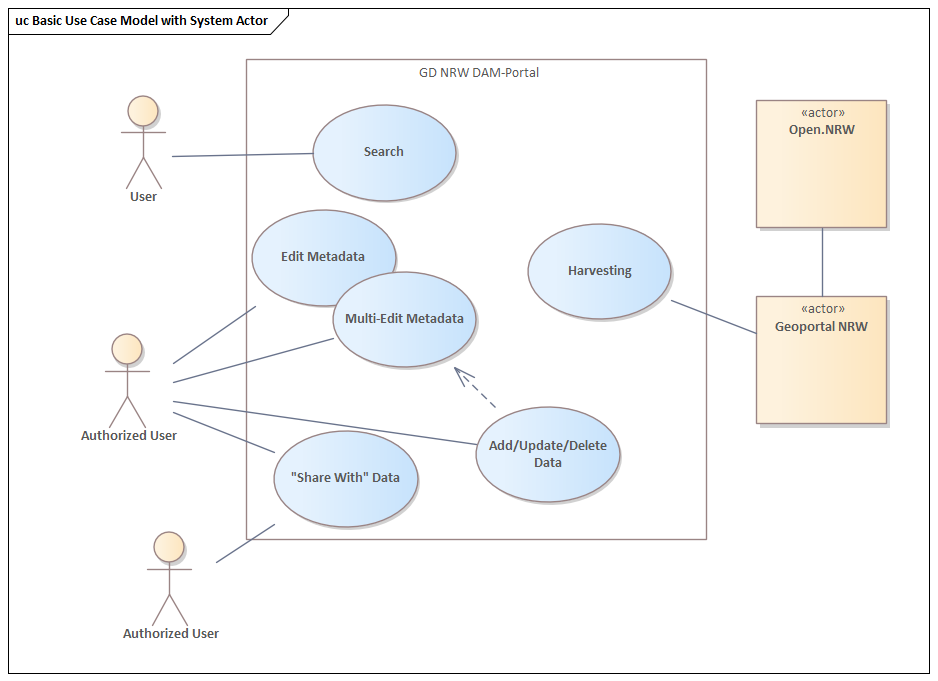
\includegraphics[width=16cm]{usecase_diagramm.png}
        \centering
    \end{figure}
    \begin{figure}[H]
        \caption{Planned software components (partial abstracted)}
        \source{con terra Internal Graphics \cite{conterraGDNRWMetaDAMPort2024}}
        \label{fig:components}
        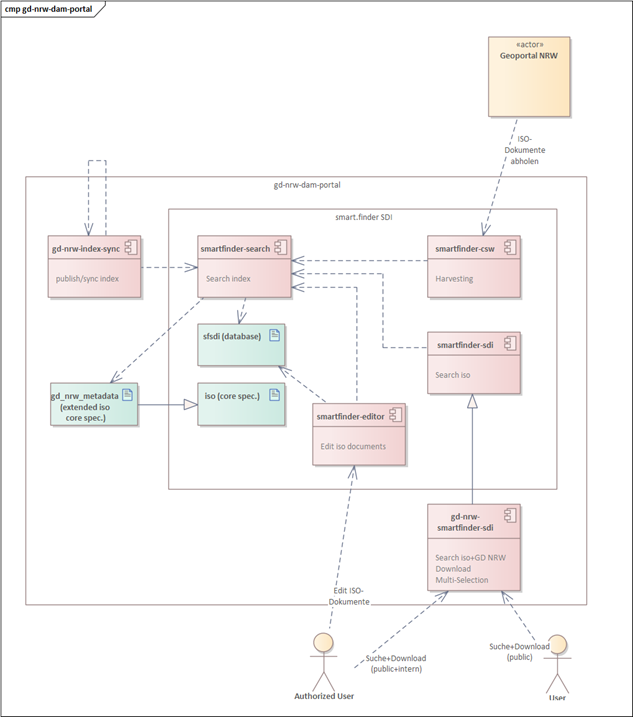
\includegraphics[width=16cm]{components_.png}
        \centering
    \end{figure}

    \begin{figure}[H]
        \caption{Planned Deployment Diagram}
        \source{con terra Internal Graphics \cite{conterraGDNRWMetaDAMPort2024}}
        \label{fig:deployment}
        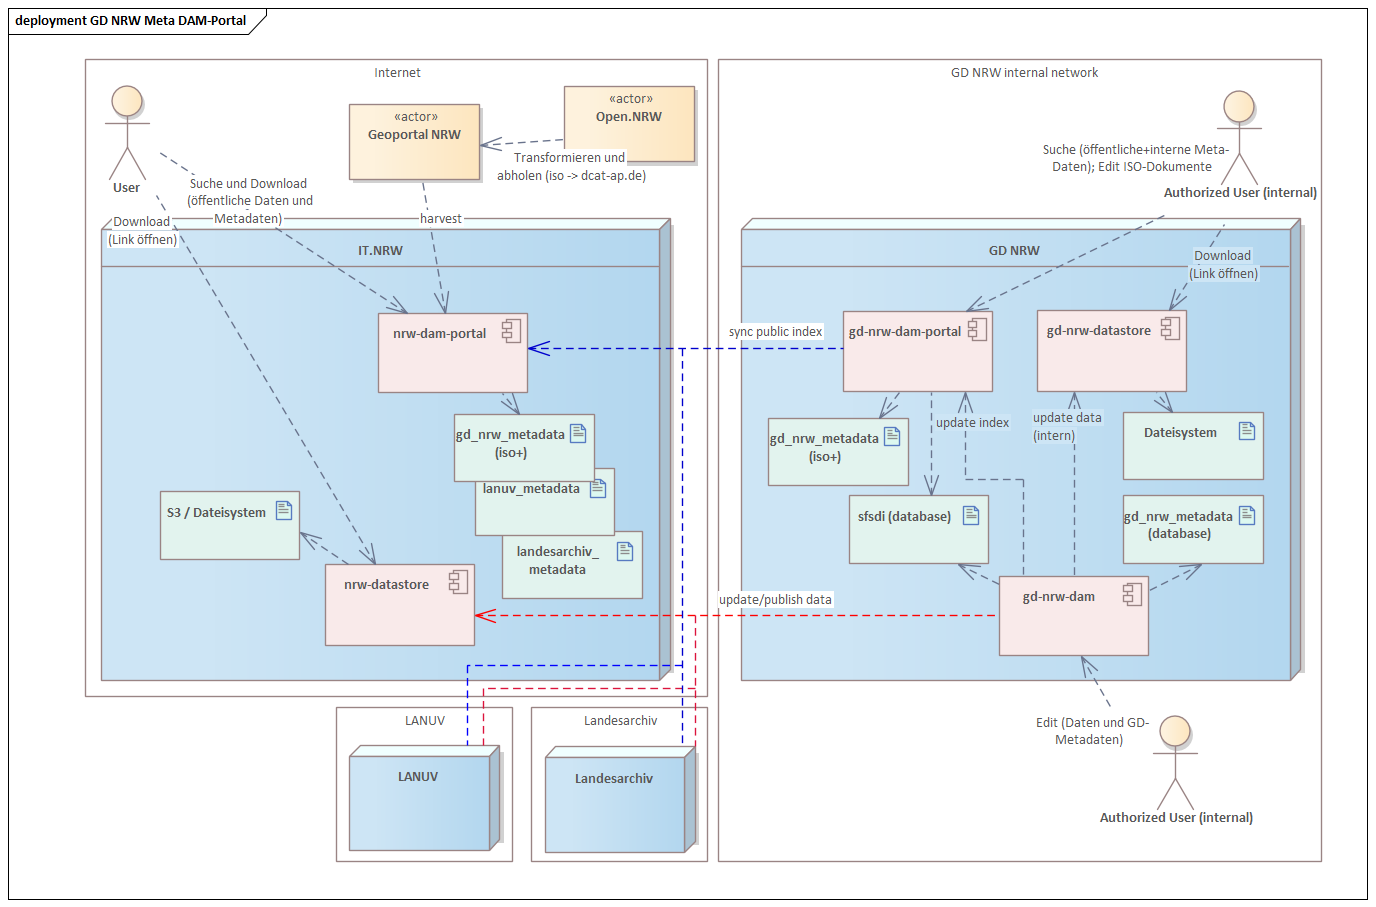
\includegraphics[width=16cm]{deployment_.png}
        \centering
    \end{figure}
    \begin{figure}[H]
        \caption{Database Scheme}
        \source{Own Graphics}
        \label{fig:db}
        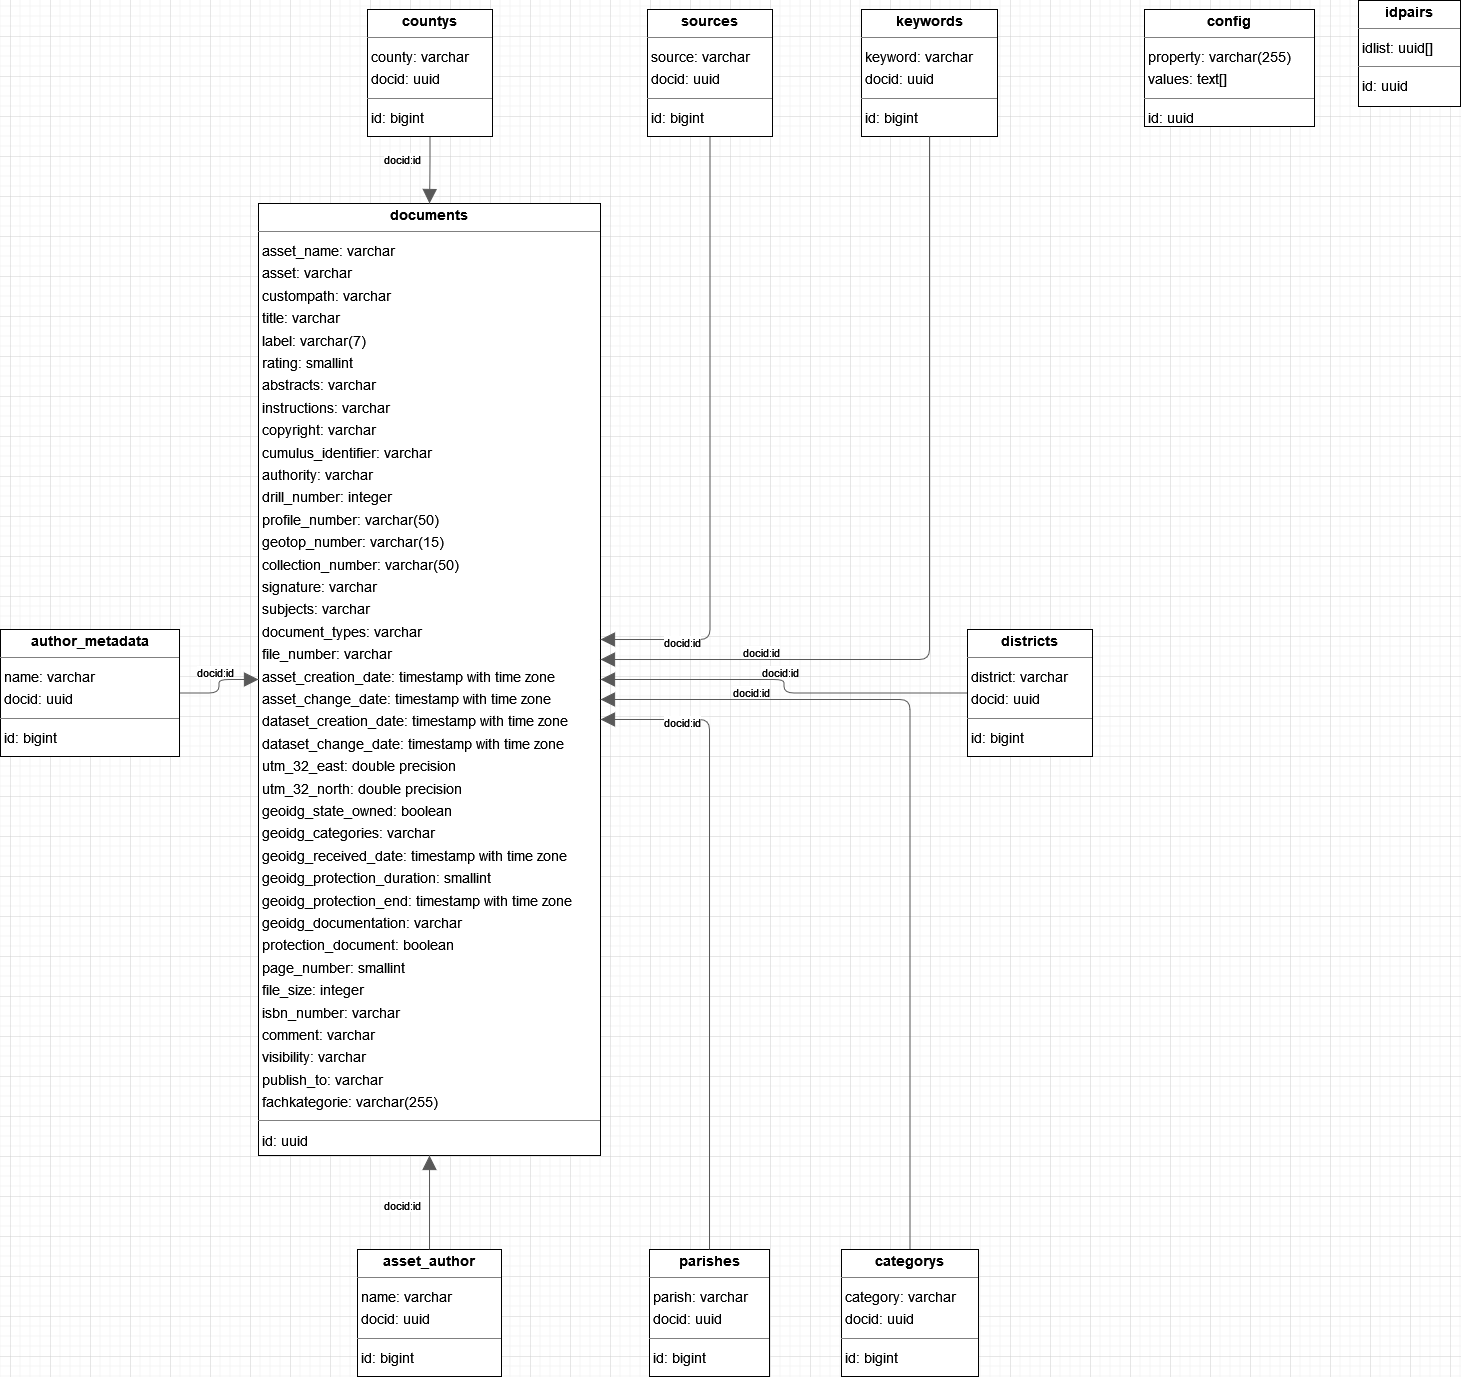
\includegraphics[width=16cm]{db3.png}
        \centering
    \end{figure}
    \begin{figure}[H]
        \caption{Screenshot Multi-Editing}
        \source{Own Graphics}
        \label{fig:multiedit}
        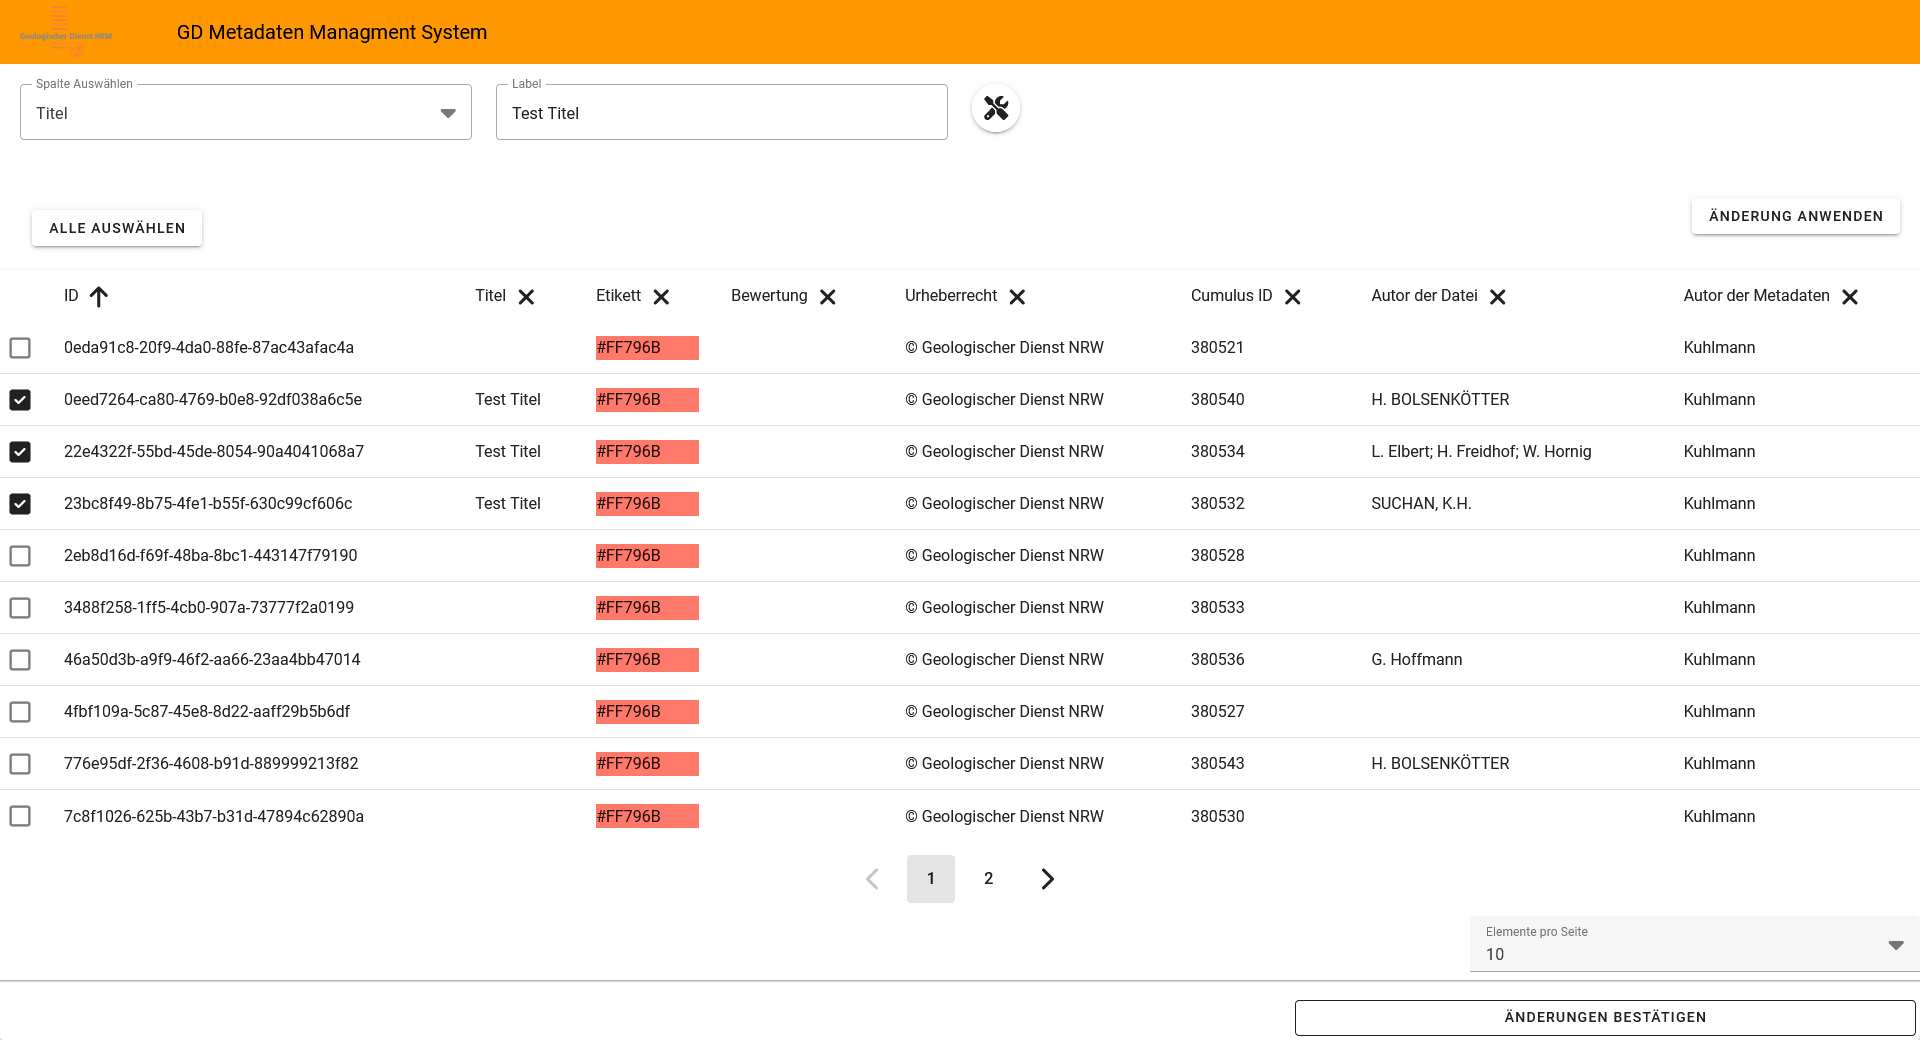
\includegraphics[width=16cm]{multiedit.png}
        \centering
    \end{figure}
    \begin{figure}[H]
        \caption{Vue Java Controller}
        \source{Own Graphics}
        \label{fig:vue}
        \begin{lstlisting}[language=java, frame=single]
        @Controller
        public class VueController {
            @RequestMapping(value = "/*/{path:[^\\.]*}")
            public String redirect(){
                return "forward:/";
            }
        }
        \end{lstlisting}
        \centering
    \end{figure}
    \begin{figure}[t]
        \caption{Fire Department Data Entry Example}
        \source{Own Graphics}
        \label{fig:pei}
        \begin{lstlisting}[frame=single]
        +CTSDSR: 108,262100112345678,1,262100188888888,1,88,1
        0A004C9CD24739C9384820
    \end{lstlisting}
        \centering
    \end{figure}

    \begin{figure}[H]
        \caption{Map Control Tool Screenshot}
        \source{Own Graphics}
        \label{fig:mapcontrol}
        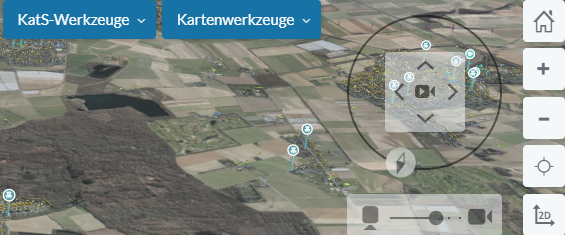
\includegraphics[width=16cm]{dzgefahr_mapcontrol.png}
        \centering
    \end{figure}
\end{appendices}



% \section{Work Experience}
% \subsection{Project Context}
% \subsubsection{Geologischer Dienst NRW - Metdata Asset Managment System}
% The  \gls {gd} NRW has a large achieve of different assets, which are currently managed by a software named cumulus. As the used software is outdated, it does not meet the the current requirements.
% Primarily they  are required to make all data, where it is legally possible, open data \cite{GesetzZurForderung2017}.
% Additionally, the GeolDG also requires the \gls{gd} to make their accessible by the public \cite{GesetzZurStaatlichen2020}.

% Therefore, the main goal of this project was to conceptualize a new system and to implement parallel a prototype of it.
% The \gls{gd} digital archive contains over 450,000 assets. Assets in this context are for example images, PDFs, TIFs or MP4s. However, any digital file can be an asset. The total data volume is over 2 terabytes.
% These assets are currently located on a shared drive and can be managed via the file system. They also use a piece of software called Cumulus. This software primarily manages the metadata associated with the assets. Currently, the \gls{gd} does not use any known metadata schema, but instead uses a list of custom attributes, such as Rating, Special Instructions and Label.
% They also use \gls{exif} and \gls{iptc} metadata information for images, which is not managed by Cumulus. Instead, this is done with an additional software component.

% The new system should eliminate the inadequacies of the old system. Therefore a list of Requirements were collected. In the following there is a subset example of the main functional requirements:
% \begin{itemize}
%     \item Keeping the Internal metadata attributes (and adding new ones)
%     \item Connection to the GEOportal.NRW
%     \item CRUD Operations for Datasets and associated metadata
%           \begin{itemize}
%               \item With an Integrated Permission System for Internal (\gls{gd} Employees) and Externals
%               \item (Multi-)Edit Interface for Metadata
%           \end{itemize}
%     \item Sharing data
%     \item Keep \gls{exif} and \gls{iptc} in sync
%     \item Syncing/Translating Internal Metadata to ISO 19115/ISO 19119
%     \item Different Search Operations
% \end{itemize}

% In addition, there are a number of quality requirements that focus primarily on data integrity and the tech stack used for development. For example, the software developed should be able to live in the cloud or on a dedicated machine.

% A final requirement is that the system needs to be split. It should mainly run on the servers of IT.NRW. But only non-sensitive data should be hosted there. Sensitive data should be hosted and only accessible by the \gls{gd} and its staff.
% \subsubsection{\gls{dz}}
% In the wake of the catastrophic flooding in Ahrtal, significant deficiencies in the hazard prevention and emergency response systems (of NRW) were exposed. Critical challenges were observed in the coordination and communication among dispatched units, such as the  \gls{thw} and the fire department. Effective communication and organization are crucial for swift and efficient emergency responses.

% Following the enactment of the "Krisenbewältigungsgesetz" in NRW in December 2022, the state government officially recognized this deficiency as an emergency situation on February 23. In response, a budget of €500,000 was allocated to address this issue.

% con terra, in collaboration with IT.NRW, submitted a proposal to develop a solution to these challenges. Their proposed solution is the creation of a digital twin, designed to aggregate and optimally visualize all relevant data for various potential scenarios. This solution aims to integrate multiple datasets from diverse sources, including the GDI-NW, LVN, and the Federal Agency for Cartography and Geodesy (BKG).
% There are currently no central systems in place to handle this kind of task. Mostly there are department specific solutions or even general purpose Systems like QGIS or ArcGIS.
% This consultancy project aims to develop a prototype which has flexible yet pivotal requirements. Some requirements were also refined and established in collaboration with fire departments during the project's course. Below is a summary of the key requirements:

% \begin{description}[]
%     \item[Three-Dimensional Capability]: Reflecting the three-dimensional nature of real-world challenges, the solution must be capable of visualizing 3D data and performing basic general-purpose operations, such as measurements, in a 3D environment.
%     \item[Scenario-Optimized Geodata]: The digital twin should tailor its data visualization and accessibility for different emergency scenarios, acknowledging that not all datasets are suitable for every scenario. Primary scenario groups include Fire, Earth, Water, and Air.
%     \item[Compliance with \gls{bhkg}]: The prototype should be developed with the objective of planning, monitoring, and follow-up in accordance with \gls{bhkg} standards.
%     \item[Target Group - Authorities and Security Organizations]: The prototype should be user-friendly for its target audience, which includes authorities and organizations involved in security tasks, without assuming extensive geospatial knowledge.
%     \item[Cloud-Based Solution]: The entire application should be cloud-based, ensuring accessibility and scalability.
%     \item[Fine-Grained Access Control]: Given the potential inclusion of sensitive data (e.g., \gls{kritis} data), the application must feature a robust access control system, allowing users to view only data relevant to their roles and responsibilities.
%     \item[Analysis Tools]: The application should offer comprehensive analysis tools. For the prototype, these will include the ability to identify and assess the accessibility of protected assets, dynamically determine water levels in 3D, and simulate the spread of smoke clouds in 3D.
%     \item[Integration of 3D Meshes]: The prototype should incorporate a detailed 3D mesh, which is currently being developed for the entire state of NRW.
%     \item[EPSG: 25832 Standard]: As a governmental project, the application must utilize the EPSG: 25832 standard for all geospatial data.
% \end{description}

% However, it is important to note that not all these requirements will be fully met in the initial phase of this project.
% \subsubsection{Geosphere}
% Geosphere is the central geoscientific institution for Austria, covering geology, geophysics, climatology, and meteorology.  It was formed by the merger of the Central Institute for Meteorology and Geodynamics (ZAMG), founded in 1851, the national meteorological and earthquake service, and the Geological Survey (GBA), founded in 1849. 
% Geosphere, needs an new Climate Atlas. They stated they need this because of EU Regulations. The new atlas should be developed by the con terra, as they were recommended. Currently the project is in the acquisition stage and i developed a prototype with few example datasets.
% %Todo: Ergänzen warum wir das machen..
% \subsection{Assigned Work}
% \subsubsection{Geologischer Dienst NRW - Metadata Asset Management System}
% My involvement in this project focused on the development of new software components for a prototype. Furthermore, I made modifications to the smart.finder SDI.


% The prototype I created was a basic project that used FastAPI and Python. It included an extra PostgreSQL database. The main goal was to design a database schema that met our needs. We chose a flat structure without any N-M relationships.
% Also, I designed the frontend. Our technological stack for the frontend consisted of Vue and Vuetify, with the inclusion of a Vite development server. The primary Vue components that I developed include Single Editing for modifying a single Metadata set and Multi-Edit for modifying multiple Metadatasets. To create Single Editing, I used a mockup as a template to base my development on. I designed, conceptualised and implemented Multi-Editing myself.

% Later on in the project, I developed an additional front-end for a shopping cart, which serves as an intermediary website between the smart.finder SDI and the new components. Moreover, I developed a front-end for the administrator to configure various attributes for editing.

% \begin{figure}[H]
%     \caption{Vue Java Controller}
%     \label{fig:vue}
%     \begin{lstlisting}[language=java, frame=single]
%         @Controller
%         public class VueController {
%             @RequestMapping(value = "/*/{path:[^\\.]*}")
%             public String redirect(){
%                 return "forward:/";
%             }
%         }

%         \end{lstlisting}
%     \centering
% \end{figure}


% After that, a decision was made to drop Python and FastAPI in favour of Spring Boot and Java. This began by implementing the required Spring Data classes and interfaces. Afterwards I began implementing the fundamental endpoints for \gls{crud} operations to restore functionality to the frontend. Additionally, the capacities to host the built front-end on the Spring Boot server were incorporated. I developed a special Spring Boot controller to keep the Vue router component of the frontend working, as it controls the routing. Incase a website should be laoded it redirects to the Vue Router and enables it to route it. The code for this can be found in \ref{fig:vue}. It should be noted that any requests that match the applied regex pattern will be directed to the Vue Router, even those that have no match in the Router.

% An Azure build pipeline was developed to enable automated deployment on our test system. This required restructuring the project into two distinct components: the frontend and the backend. Each component is now a complete Maven project, with its own pom.xml file. Furthermore, the entire project is encapsulated in a separate Maven project, which also has its own pom.xml file. The Maven arrangement enables the project to be built with the fully integrated frontend and backend, specifically tailored for the pipeline. To deploy to our test machine, we utilized the tomcat-maven-plugin.

% Later, I developed an additional API component. It is a Spring Boot application that accesses the smart.finder SDI and alters its Solr database. During development, I extended the smart.finder SDI Solr core to handle additional attributes beyond ISO. Moreover, I enhanced the frontend of the smart.finder SDI to display those attributes.
% Also i created an automated ISO XML generation based on our new attributes.

% Finally, I have developed several complex features, including thumbnail generation for images and PDFs, on-the-fly zipped group downloads, \gls{iptc}/\gls{exif} read and write capabilities, and the deployment of a Redis Instance for fast and secure storage. This addition will facilitate the transition from the smartfinder to the new components. Also i deployed an Nginx instance as a reverse proxy for basic authentication, with TLS support.


% \subsubsection{\gls{dz}}
% I joined the project during its final stages and focused on a limited but significant set of tasks. My primary responsibility involved integrating data provided by the fire department. I worked with a PEI Dataset, which consisted of radio messages containing location data, such as Short PDU, Long PDU, or STATUS. An example of this data is shown in Figure \ref{fig:pei}. The first line of each message includes metadata, like the transmitting and receiving parties, and the message type. The HEX-Code following this metadata can be converted to binary and decoded according to the ETSI TS 100 392-18-1 standard. I developed a Python script to automate this process, outputting the data as an ESRI feature layer.

% \begin{figure}[H]
%     \caption{Fire Department Data Entry Example}
%     \label{fig:pei}
%     \begin{lstlisting}[frame=single]
%         +CTSDSR: 108,262100112345678,1,262100188888888,1,88,1
%         0A004C9CD24739C9384820
%     \end{lstlisting}
%     \centering
% \end{figure}

% Additionally, I developed a new map control tool, enhancing user interaction with map features such as position, rotation, tilt, and zoom. This tool allows users to intuitively adjust the map's rotation by dragging the north arrow around a circle, as illustrated in Figure \ref{fig:mapcontrol}.

% \begin{figure}[H]
%     \caption{Map Control Tool Screenshot}
%     \label{fig:mapcontrol}
%     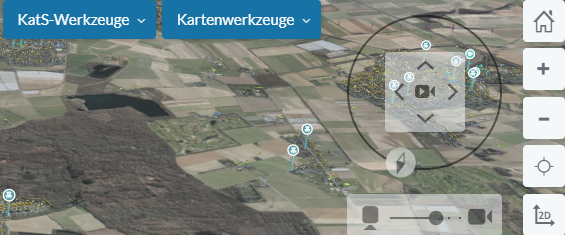
\includegraphics[width=16cm]{dzgefahr_mapcontrol.png}
%     \centering
% \end{figure}

% I also improved the animation of moving objects in map.apps, particularly for a layer that displays live bus positions in Münster. Previously, buses would appear to 'teleport' across the map; my update, using the animejs library, enabled smooth motion during position updates.

% My final task was to assess the compatibility of Esri's ArcGIS Indoors Technology with mapapps. The evaluation concluded that compatibility is currently limited.
% \subsubsection{Geosphere}
% For this project, I primarily developed a prototype that can be presented. The prototype was based on a map.apps project.    I received multiple datasets with \gls{rcp} Scenarios (RCP 2.6, RCP 4.5, RCP 8.5) that were split into two types: timeseries data and median data. The median datasets only contained the median value for a given period for the entirety of Austria. The dataset includes complete model simulations and associated statics for Austria, presented in rasterized 1000 x 1000m blocks. The variable measured is 'SU30', representing the number of days with temperatures over 30 degrees Celsius.
% The median data was visualized in map.apps and a user interface was developed to provide more intuitive control over the displayed data. In addition, I developed a Python backend and frontend to enable the visualization of time series data in map.apps. The Python backend was based on FastAPI and accessed the datacubes directly. The frontend creates plots on the fly using Plotly. Finally, I created a reporting function that allows the user to generate a report based on the selected data. The data is then aggregated into a PDF that can be printed.



% \subsubsection{Study Relevant Competencies}
% During my internship, I applied concepts and skills from my academic curriculum in Geoinformatics and Spatial Data Science. The internship required me to use my software development competencies, which I developed through various modules in my study program. The internship required the development of software components using programming languages such as JavaScript, Java, and Python. Basic database management competencies, which were also a part of my academic training, proved to be highly valuable in addition to these programming skills.

% However, it is important to note that my university curriculum did not cover certain aspects that were essential to my internship. Specifically, the use of Frontend Frameworks such as React, Angular, or Vue, as well as other practical applications of frameworks and libraries in these programming languages were not addressed. As a result, I had to learn on my own to become proficient in these areas.

% Moreover, I did not receive formal education on the use of Object-Relational Mapping (ORMs) for database access, a critical component in modern software development, which was extensively utilized during my internship. Furthermore, the planning and development of complex and complete infrastructures, which are pivotal in large-scale software projects, were not covered in my academic syllabus.

% Furthermore, my formal education did not cover advanced concepts such as Reverse Proxies and Secure Sockets Layer (SSL) encryption, which are crucial for ensuring secure and efficient web communication. Additionally, I did not receive any instruction on the application of Geographic Information Systems (GIS) in the context of 3D environments.

% % In summary, my academic background in Geoinformatics and Spatial Data Science provided a strong foundation in software development and basic database management. However, my internship experience highlighted the need for a more expansive curriculum that includes practical applications of modern software frameworks, advanced infrastructure planning, and the integration of GIS in 3D modelling. This will better prepare students for the evolving demands of the industry.

% \subsubsection{The state of planning}
% Afterwards, I was supposed to be involved in the Open Pioneer track, where I would integrate 3D functionalities using DeckGL to enhance its capabilities. However, it was later reassessed and deemed infeasible. 
% As a result, my internship took a different direction, and I was reassigned to work on the DZGefahr project for a few months. Following this, I developed the Geosphere prototype.

% \section{Results Obtained}
% The evaluation of my internship work was carried out using a methodology that differed from traditional report-based evaluations; the evaluation process was more incremental and continuous, rather than resulting in a formal report.

% Feedback was primarily given through direct interactions with other developers, project leads, and user experience (UX) designers. The mechanism for feedback was informal and integrated into the daily workflow. It did not involve structured meetings solely for performance evaluation. Instead, feedback was integrated into the collaborative process, offering immediate and practical insights into the quality and relevance of contributions.

% When a feature was considered acceptable, it was marked as complete. The primary tool for tracking progress and organizing tasks was the use of Jira boards.

% In addition to this ongoing feedback mechanism, I had bi-weekly discussions with my supervisor. These meetings served as a platform to evaluate not only the current state of specific projects I was working on but also the overall progression of my internship experience.

% \section{Project contributions}
% As my work was primarily focused on developing prototypes, I could not see any contributions to a larger project. Instead, most of the things I did will hopefully become part of a larger project at a later stage, as my prototypes were primarily used for acquisition purposes.

% \section{Communication competences}
% In the following i will describe various Communication competencies in a short way.
% \begin{description}[]
%     \item[Supervisor Communication:] As previously stated, I had bi-weekly meetings with my supervisor. These were scheduled meetings.
%     \item[Teamwork:] I was part of the team, but because teams do not work together on a project, I did not really get to know each team member. Instead, I had regular contact with individuals who worked on the same project. However, as my tasks were mostly isolated, I worked independently without a team.
%     \item[Professional Network:] As I had already worked for two years prior to my internship at con terra, I did not expand my professional network in any way.
%     \item[Conflicts:] There were no conflicts during my internship that involved me.
%     \item[Communication Skills:]  During my internship, I did not acquire any new communication skills related to working on large-scale projects beyond prototypes. However, I did attend career services seminars where I learned a few new skills.
%     \item[Applied Communication Skills:]  As the general workflow and interaction in con terra are very similar to those in the university, I could easily adapt.
% \end{description}

% \section{Master Thesis Implications}
% The internship experience did not provide topics that would align with the requirements or themes suitable for a Master's thesis. However, I proactively addressed this by discussing potential thesis topics with my supervisor within the broader scope of the organization's interests and projects.

% The discussions centred on Wind Turbine Placement, a subject of growing interest and relevance in sustainable energy and spatial planning. con terra has expressed a clear interest in this topic. The federal states are actively seeking software solutions to simplify and optimise the process of placing wind turbines. This aligns with con terra's ambitions for a digital twin.

% A digital twin involves creating a virtual replica of a physical entity or system, offering a sophisticated approach to analyzing and optimizing wind turbine placement. This approach can contribute significantly to the efficient and sustainable development of wind energy resources, which is critical for environmental sustainability and energy transition.

% Currently, the idea of focusing a Master's thesis on this topic is in its early stages and has not been definitively decided. It is still a concept under consideration, and its potential and feasibility have yet to be fully explored and confirmed. This ongoing discussion reflects the dynamic nature of academic and professional exploration, where ideas evolve and are refined over time, in alignment with both academic objectives and the practical needs of the industry.

% \section{Learning Goals}
% In the following I will list each Learning Goal and evaluate if it was reached in the course of the internship

% \begin{description}[]
%     \item[Enhancement of proficiency in GIS software and infrastructure:]  This learning goal has been fully achieved. I have deepened my expertise in desktop GIS software, such as ArcGIS Pro, as well as on the server side with ArcGIS Server infrastructure. Additionally, I have gained experience in developing web GIS applications using the ArcGIS JS SDK and map.apps. I have also worked with various dataset types, including PEI datasets, file geodatabases, and NetCDF. 
%     \item[Further development of coding and data analysis capabilities:] This learning objective was fully achieved. I have developed several different applications in several languages. For example, I developed a complete Spring Boot app with a SQL database. I also developed some Python components and several JS applications for map.apps. In the context of data analysis I have a lot of experience with netCDF files and ArcGIS and Python.
%     \item[Mastery in data management]: Not archived. Although my internship had parts of data analysis, it was never the main focus. Data management consisted mainly of converting any data into an ArcGIS format and publishing it to an ArcGIS server. I also used flat structures for files that could not be converted to ArcGIS compatible formats.
%     \item[Acquisition of knowledge in emerging technology standards:] Partially archived. Even though I did not learn any extremely new technology, I did learn a lot of new technologies and how to use them. For example: Vue(3), SpringBoot, Nginx and Redis.
%     \item[Familiarization with project management and participation in large-scale projects:] Not archived. I did not work on any large-scale projects during my internship.
%     \item[Development of collaborative skills for team environments:] Archived. I have had some experience of working with real teams. Especially in the GD NRW project.
%     \item[Improvement in effective communication strategies:] Not archived, as i did not work enough in teams.  
%     \item[Skill development in recognizing correlations between various topics:] As I only visited a few projects, I was not able to make any real connections.
%     \item[Improvement in strategizing for problem-solving:] Archived. As I encountered many different problems, I learned new strategies to solve them.
% \end{description}

% I achieved four out of nine goals, which I still consider a success. The goals that were not met were too abstract unrealistic, or not fitting for con terra. Therefore, one of the most important things I learned from the internship is what to expect and what not to expect when working in the industry.

% \section{Summary and conclusions}

% My internship at con terra was, in my opinion, a successful first experience in the industry. I gained knowledge in the applied usage of new technologies and deepened my understanding of technologies I was already familiar with. Additionally, I acquired new social skills, such as working in small teams, and further developed my soft skills. During my internship, I had the opportunity to develop my soft skills while working in the office and interacting with colleagues. 
% For my future studies, I do not believe that my internship will provide significant benefits. However, as my studies are coming to an end, it is likely that I will remain at con terra. 


\clearpage


\clearpage
\printglossary[type=\acronymtype]
\printglossary
\clearpage
\printbibliography

\end{document}
